\section{The Cube as a Group}
\label{Chapter_CubeAsGroup}

In this section, the group of the \Ttwo cube is defined. First, the rotation of the cube and the equality of two moves are understood using equivalence relations and equivalence classes. This is necessary so that the same moves do not appear twice in the group's generating set. Identical moves are then represented by an equivalence class.

Basically, I tried applying the notions and understandings of the \Tthree \textit{Cube} \cite{JC} to \Ttwo \textit{Cube}.
To do this, the group of the \Ttwo cube is examined for the four group axioms (closure, associativity, existence of identity, and existence of an inverse element). It is also checked whether it is an abelian group or not and then the commutativity is examined. A group operation for making moves is then defined on the group of the \Ttwo cube. The order of permutations and moves and the equivalence of moves are also calculated.

\subsection{Equality of Moves}
\label{Section_EqualityOfmoves}

\begin{definition}
  $A_Z$ is defined as the infinite set of all moves of the cube.  
\end{definition}
\begin{definition}
Two moves $Z_1$ and $Z_2 \in A_Z$ are considered equal if they produce the same final configuration with the same initial configuration of the cube.
\end{definition}
A move consists of one or more basic moves ($U, D, R, L, F, B$).

\begin{notation}
 Executing moves multiple times can be represented using exponent notation. For example, $RR$ (two rotations of the right face clockwise) is  written as $R^2$. The exponent notation can be used for all moves, even if they rotate more than one face. For example, the move $(LLFF)^2$  corresponds to $LLFFLLFF$.   
\end{notation}

We'll now consider the equality of moves in details.
\textbf {If a face is rotated four times in a row, the cube is back in the previous position. If the cube is in any configuration $C = (\sigma, x)$ and a move $Z \in \{ U^4, D^4, R^4, L^4, F^4, B^4 \}$ is executed, the resulting configuration is again $C$} $\forall \ Z \in \{ U, D, R, L, F, B\} \\ $:
\begin{align*}
C \cdot Z^4 = C
\end{align*}
This means that each move $Z = Z_1Z_2Z_3$ with $Z_2 \in \{ U^4, D^4, R^4, L^4, F^4, B^4\}$ has the same configuration as the move $Z_1Z_3$ causes.
In this case, the exponent can be calculated modulo 4, since four rotations of a face one after the other lead back to the starting state.
It, therefore, applies to all configurations $C$ of the cube $\forall \ Z \in \{U, D, R, L, F, B\}, n \in \mathbb{N} $:
\begin{align*}
 C \cdot Z^n= C \cdot Z^{n \hspace*{-0.5em} \mod 4}
\end{align*}
This is true because each face rotation ($U, D, R, L, F$ or $B$) is defined by a permutation function $\sigma$. For each of these basic features, $\sigma$ consists of only one four-element cycle \ref{Section_PositionsOfThecubiesInTheCube} (cycle of length 4 ).  After four executions of a four-element cycle, it returns to its original state ( discussed in more details in \ref{Section_OrderPermutations}). In addition, the vector $x$ must be taken into account for the orientation of the cubies. This vector is changed by a function $\gamma$. The vector $x$ always returns to its initial state if the same function $\gamma$ is executed four times in a row. 
%This is shown in Appendix \ref{Appendix_Alignment Functions} for all basic features of the cube.


For any cube configuration $C$ and all $n$ that are multiples of four, then:
\begin{align*}
\forall \ Z \in \{U, D, R, L, F, B\}, n \in \mathbb{N}, n \hspace*{-0.6em} \mod 4 = 0 \ . \
C \cdot Z^n
= C
\end{align*}
In this case, we can carry out the following transformation:
\begin{align*}
C \cdot Z^n
= C \cdot Z^{n \hspace*{-0.5em} \mod 4}
= C \cdot Z^0
= C
\end{align*}
$Z^0$ represents an empty move. This does not correspond to any change in the resulting configuration of the cube.

Since, the number of possible moves ($|A_Z|$) is infinite, in contrast to the number of valid cube configurations (discussed in \ref{Chapter_ValidConfigurations}), there are infinite number of cases in which two moves produce the same resulting configuration and are ,therefore, considered equal. 

\subsection{Rotation of the Cube}

\label{Section_RotationOfCube}

In contrast to the \Tthree cube, the \Ttwo cube has no center cubies that determine how the cube is aligned.
The \Ttwo cube can, therefore, be in the solved state without the top side being white. Therefore, it must be possible to rotate the cube completely.
This should be implemented as an equivalence relation in section \ref{Section_EquivalenceRelationOfMoves}. For this purpose, the rotation options of the cube are defined in this section.
To name the rotations, the axes of the cube are defined as $x, y$ and $z$. This can be seen in Figure \ref{Image_Axes of Rotation}. The vertical axis is called $z$. The $x$ axis runs from front to back through the cube and the $y$ axis runs from right to left.
\begin{figure}[H]
\centering
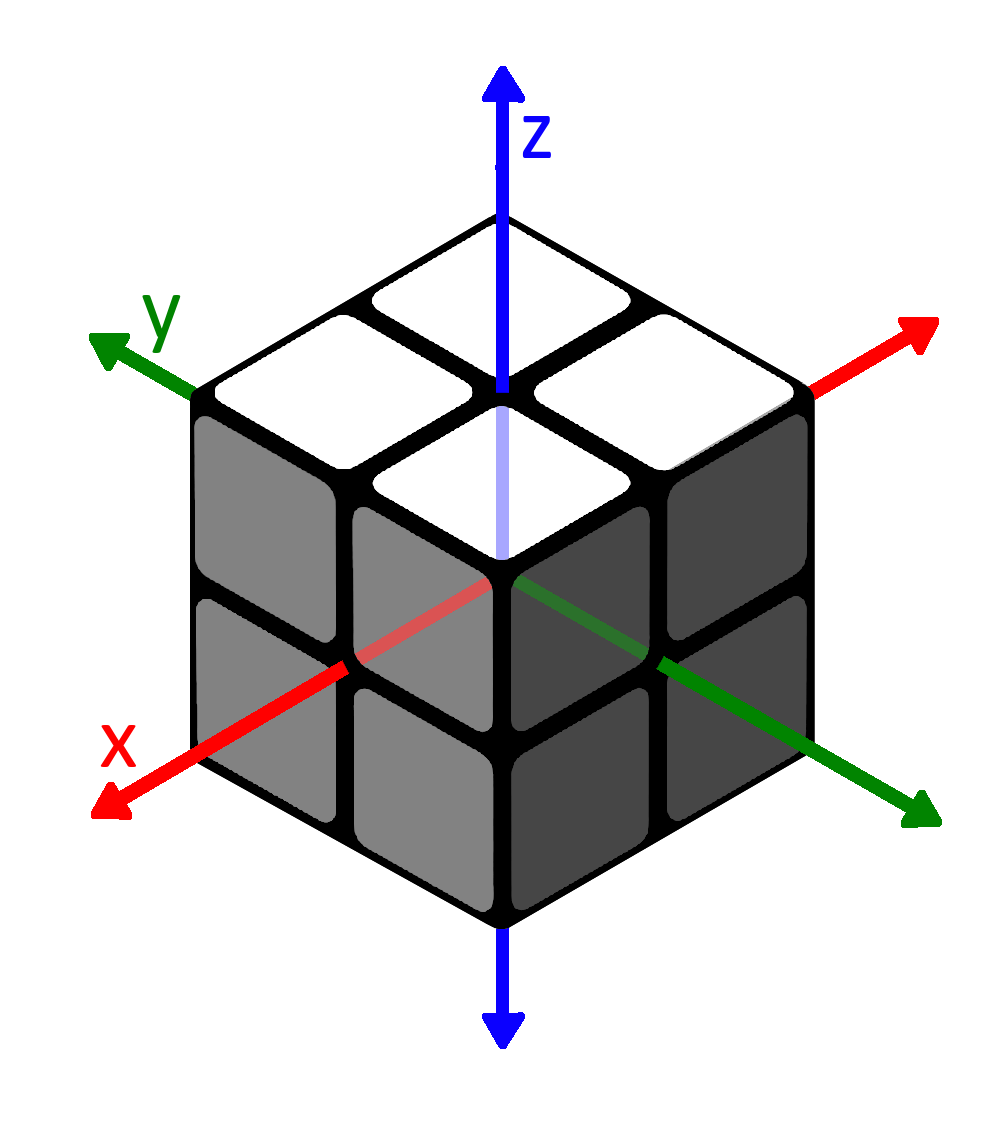
\includegraphics[scale=0.13]{Axis.png}
\caption[Cube with $x, y$ and $z$ axes]{Cube with $x$, $y$ and $z$ axes}
\label{Image_Axes of Rotation}
\end{figure}

The designations of the axes can be used to define resulting configurations for the possible rotations of the cube.
To do this, the individual rotations of the cube are first named. These are 90$^\circ$ rotations.

\vspace*{1em}
\begin{adjustbox}{width=1\textwidth,center}
\begin{tabular}{cl}
\toprule
\textbf{Notation} & \textbf{Description of rotation} \\
\midrule
$Z_l$ & rotation of the cube around the $z$ axis to the left (counterclockwise)\\

$Z_r$ & rotation of the cube about the $z$ axis to the right (clockwise) \\

$Y_l$ & rotation of the cube around the $y$ axis to the left (counterclockwise)\\

$Y_r$ & rotation of the cube about the $y$ axis to the right (clockwise) \\

$X_l$ & rotation of the cube around the $x$ axis to the left (counterclockwise)\\

$X_r$ & rotation of the cube about the $x$ axis to the right (clockwise) \\

$N_R$ & no rotation of the cube \\
\bottomrule
\end{tabular}
\end{adjustbox}

\vspace{0.5cm}
 There are only four rotation options for each side of the cube ($0^\circ, 90^\circ, 180^\circ, 270^\circ$), since it is always rotated by $90^\circ$. For example, $Z_l$ is the same as ${Z_r}^3$. This means that one 90$^\circ$ rotation of the cube to the left is equivalent to three 90$^\circ$ rotations of the cube to the right. Turning to the left equals $0^\circ-90^\circ = 270^\circ$ while three turns to the right $0^\circ+90^\circ+90^\circ+90^\circ=270^\circ$ are equivalent.

The cubies are all moved to a new position by rotating. Unlike rotating layers, where a selection of cubies changes position, here all cubies change position. The resulting configuration of the cube after a rotation is then a different equivalent configuration.

We'll now try to see the change in cubie positions as we apply the rotation $Z_r$, i.e. a rotation of the entire cube around the $z$ axis by $90^\circ$ clockwise. The cube is shown in Figure \ref{Figure_CubeAfterRotationAroundZAxis} after rotation $Z_r$.
\begin{figure}[H]
\centering
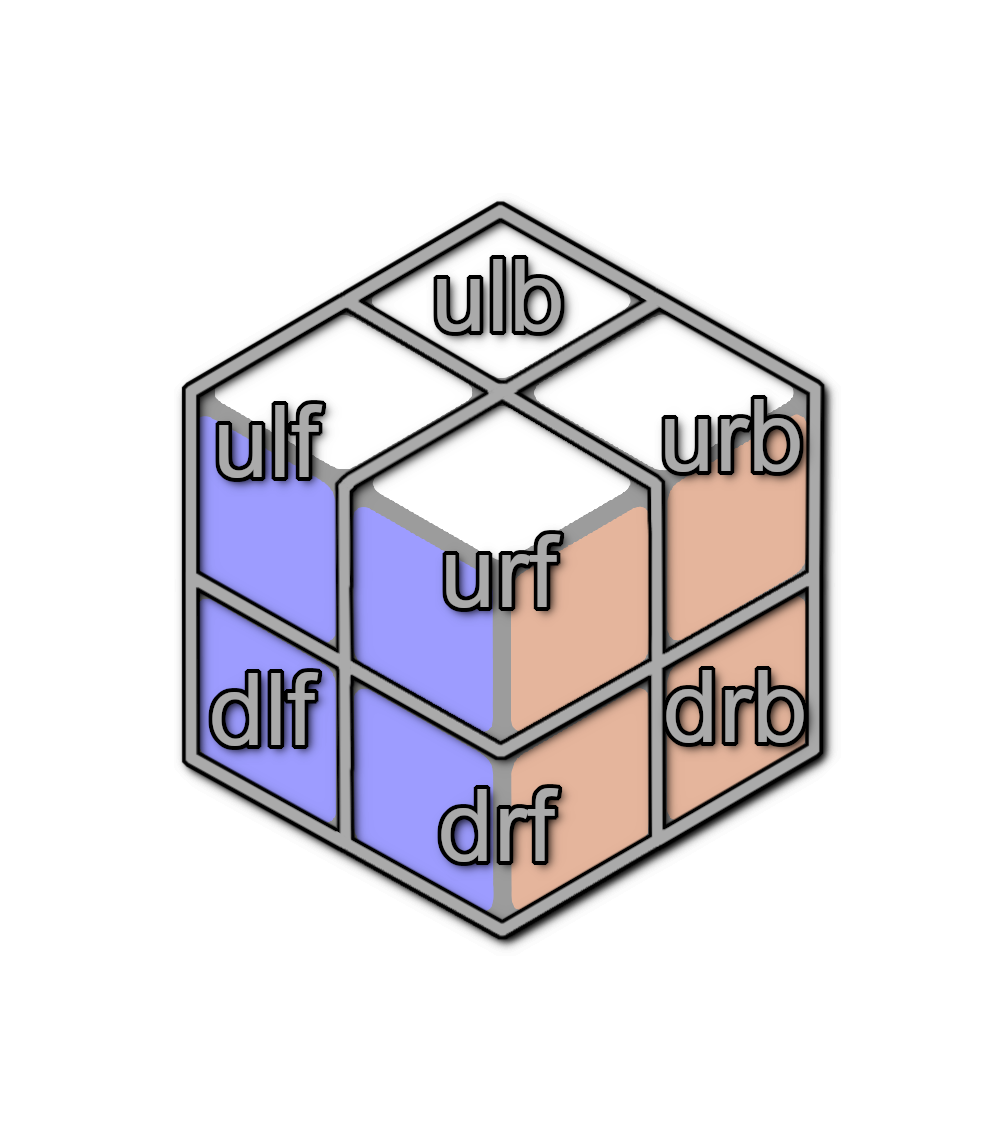
\includegraphics[scale=0.13]{on_ulf.png}
\caption{Cube after rotation around $z$-axis}
\label{Figure_CubeAfterRotationAroundZAxis}
\end{figure}
The permutation function of the rotations, from now onwards, is called $\delta$. Since, all the cubies change position during rotations, there must be a function $\delta$ for each rotation that maps each of the eight corner cubies to another:
\begin{alignat*}{4}
& \delta_{Z_r}(\textit{urf}) = \textit{ulf} \ \ \ \ \ \ && \delta_{Z_r}(\textit{ulf}) = \textit{ulb} \ \ \ \ \ \ && \delta_{Z_r}(\textit{ulb}) = \textit{urb} \ \ \ \ \ \ && \delta_{Z_r}(\textit{urb}) = \textit{urf} \\
& \delta_{Z_r}(\textit{drf}) = \textit{dlf} \ \ \ \ \ \ && \delta_{Z_r}(\textit{dlf}) = \textit{dlb} \ \ \ \ \ \ \ && \delta_{Z_r}(\textit{dlb}) = \textit{drb} \ \ \ \ \ \ && \delta_{Z_r}(\textit{drb}) = \textit{drf}
\end{alignat*}

The equivalent notation in the form $i \mapsto j$ is:
\begin{alignat*}{4}
& \textit{urf} \mapsto \textit{ulf} \ \ \ \ \ \ \ \ && \textit{ulf} \mapsto \textit{ulb} \ \ \ \ \ \ \ \ && \textit{ulb} \mapsto \textit{urb} \ \ \ \ \ \ \ \ && \textit{urb} \mapsto \textit{urf} \\
& \textit{drf} \mapsto \textit{dlf} \ \ \ \ \ \ \ \ && \textit{dlf} \mapsto \textit{dlb} \ \ \ \ \ \ \ \ && \textit{dlb} \ mapsto \textit{drb} \ \ \ \ \ \ \ \ && \textit{drb} \mapsto \textit{drf}
\end{alignat*}

In cycle notation, the function $\delta_{Z_r}$ for the rotation $Z_r$ corresponds to the following expression:
\begin{align*}
\delta _{Z_r}=( \textit{urf} \ \textit{ulf} \ \textit{ulb} \ \textit{urb} )\ ( \textit{drf} \ \textit{dlf} \ \textit{dlb} \\textit{drb} )
\end{align*}
 

The remaining rotations can also be represented by functions $\delta$ in cycle notation. The empty rotation is identity. The functions $\delta$ for all rotations are listed below:

\begin{alignat*}{2}
& \delta_{Z_r} && = ( \textit{ulf} \ \textit{ulb} \ \textit{urb} \ \textit{urf})\ (\textit{dlf} \ \textit{dlb} \ \textit{drb} \ \textit{drf} )\\
& \delta_{Z_l} && = ( \textit{ulf} \ \textit{urf} \ \textit{urb} \ \textit{ulb})\ (\textit{dlf} \ \textit{drf} \ \textit{drb} \ \textit{dlb} )\\
& \delta_{Y_r} && = ( \textit{ulf} \ \textit{ulb} \ \textit{dlb} \ \textit{dlf})\ ( \textit{urf} \ \textit{urb} \ \textit{drb} \ \textit{drf} )\\
& \delta_{Y_l} && = ( \textit{ulf} \ \textit{dlf} \ \textit{dlb} \ \textit{ulb})\ ( \textit{urf} \ \textit{drf} \ \textit{drb} \ \textit{urb} )\\
& \delta_{X_r} && = ( \textit{ulf} \ \textit{urf} \ \textit{drf} \ \textit{dlf})\ ( \textit{urb} \ \textit{ulb} \ \textit{dlb} \ \textit{drb} )\\
& \delta_{X_l} && = ( \textit{ulf} \ \textit{dlf} \ \textit{drf} \ \textit{urf})\ (\textit{urb} \ \textit{ulb} \ \textit{dlb} \ \textit{drb} )\\
& \delta_{I_R} && = \ 1 \hspace*{14.1em}
\end{alignat*}
Since the rotations transform an arbitrary cube configuration into another equivalent cube configuration, so in addition to the permutation functions for changing the position of the cubies, there must also be transition functions for the vector $x$, which represents the orientation of the cubies. The functions $\gamma$ have already been defined and described for each move of the cube ($U, D, R, L, F, B$) in section \ref{Section_AlignmentOfcubies}. Just the vector entries of the cubie alignments were changed there with the functions $g, h$ and $i$.
\begin{align*}
g(x)=(x + 2) \hspace*{-0.5em} \mod 3 \ \ \ \ \ h(x) = (x+1) \hspace*{-0.5em} \mod 3 \ \ \ \ \ i(x)=x
\end{align*}

The transformation functions of the vector $x$ are, from here, we call $\beta$. For each of the rotations, there is a function $\beta$ that transforms the vector into its resulting state. The identity function $i$ needs not to be listed. The functions $\beta$ for the rotations are defined below:
\begin{align*}
\beta_{Z_r}  & \left( (x_1, x_2, x_3, x_4, x_5,x_6,x_7,x_8) \right) = (x_3, x_1, x_4, x_2, x_7, x_5, x_8, x_6) \\
\\
\beta_{Z_l}  &   \left( (x_1, x_2, x_3, x_4, x_5,x_6,x_7,x_8) \right)  = (x_2, x_4, x_1, x_3, x_6, x_8, x_5, x_7) \\
\\
\beta_{Y_r}  &  \left( (x_1, x_2, x_3, x_4, x_5,x_6,x_7,x_8)  \right) =  (h(x_3), g(x_4), g(x_7), h(x_8), g(x_1), h(x_2), h(x_5), g(x_6)) \\
\\
\beta_{Y_l}  &   \left( (x_1, x_2, x_3, x_4, x_5,x_6,x_7,x_8) \right)  = (h(x_5), g(x_6), g(x_1), h(x_2),g(x_7),h(x_8),h(x_3),g(x_4)) \\
\\
\beta_{X_r}  &  \left( (x_1, x_2, x_3, x_4, x_5,x_6,x_7,x_8)  \right) = \ (g(x_5), h(x_1), h(x_7), g(x_3), h(x_6), g(x_2), g(x_8),h(x_4)) \\
\\
\beta_{X_l}  &  \left( (x_1, x_2, x_3, x_4, x_5,x_6,x_7,x_8) \right)  =  (g(x_2), h(x_6), h(x_4),g(x_8), h(x_1), g(x_5), g(x_3), h(x_7)) 
\end{align*}
If the cube is not rotated, the vector $x$ remains unchanged. The function $\beta$ for the empty rotation $N_R$ is defined below:
\begin{align*}
\beta_{N_R} & \left( (x_1, x_2, x_3, x_4, x_5,x_6,x_7,x_8) \right) = (x_1, x_2, x_3, x_4, x_5,x_6,x_7,x_8)
\end{align*}

Multiple rotations can also be carried out one after the other. The functions $\delta$ and $\beta$ are then each nested. This is done in the same way as executing moves multiple times.

When looking at the rotations and the associated functions, it is noticeable that the rotations can also be defined by a combination of moves. \newpage The rotations correspond to the following moves:
\begin{alignat*}{3}
& Z_l && \Leftrightarrow \ \ && D U^{-1} \\
& Z_r && \Leftrightarrow && D^{-1} U \\
& Y_l && \Leftrightarrow && L R^{-1} \\
& Y_r && \Leftrightarrow && L^{-1} R \\
& X_l && \Leftrightarrow && B F^{-1} \\
& X_r && \Leftrightarrow && B^{-1} F \\
& I_R && \Leftrightarrow && N
\end{alignat*}
Each rotation can therefore be represented by the face rotations of two opposite sides of the cube.

\subsection{Maximum Number of Rotations}
\label{Section_MaxNumberRotations}

Executing a rotation multiple times is also written using exponent notation.
Thus, for any one-element rotation $T$ and any configuration $C$:
\begin{align*}
\forall \ T \in \{{Z_r}, {Z_l}, {Y_r}, {Y_l}, {X_r}, {X_l} , I_R \} \ . \ C \cdot TTTT= C \cdot T^4=C \cdot N_R = C
\end{align*}
Where $N_R$ is the empty rotation and $T$ is any rotation of the cube. This therefore applies to any rotation $T$:
\begin{align*}
T^{\hspace*{0.1em}0}=N_R
\end{align*}
Every one-element rotation is defined by the functions $\delta$ and $\beta$. Each of these functions $\delta$ consists of two 4-cycles. These cycles return to their initial state after four executions.  In addition, with each rotation the vector $x$ is changed by a function $\beta$. The vector remains unchanged after executing $\beta$ four times. 
The proof of this can be found in appendix \ref{Appendix_AlignmentFunctions}.
Since, all quadruples of the one-element rotations (${Z_r}, {Z_l}, {Y_r}, {Y_l}, {X_r}, {X_l} , N_R$) do not cause any change, the exponent of the rotations can be calculated modulo 4. Where $C$ is any cube configuration:
\begin{align*}
\forall \ T \in \{{Z_r}, {Z_l}, {Y_r}, {Y_l}, {X_r}, {X_l}, N_R \}, n \in \mathbb{N} \ . \ C \cdot T^n=C \cdot T^{n \hspace*{-0.5em} \mod 4}
\end{align*}

From this statement, it can be seen that the cube can return to its original orientation after several rotations. Therefore, there is a maximum number of rotations, with each additional rotation returning the cube closer to its original state.
Here, we'll see the maximum number of times the cube must be rotated by 90$^\circ$ to return to its original rotation. In the initial configuration, the white side is up.

Since the cube has six sides, each of which can have four different orientations, there are $4 \cdot 6 = 24$ different rotation possibilities for the cube. Figure \ref{ImageCubeRotationWhiteSide} shows the four different orientations of the cube when the white side is assumed to be the top side. We take a solved cube. There are also four alignment options for the other five colours. 

\begin{figure}[H]
\centering
\includegraphics[scale=0.063]{RotationWhite.png}
\caption{Rotation possibilities of the cube with the white side up}
\label{ImageCubeRotationWhiteSide}
\end{figure}
In addition to the illustrations of all possible rotations of the cube, there is a table in the appendix part \ref{Appendix_RotationsOfCube} that shows all rotations and the links between them. Using this complete representation of the rotation possibilities, it can be determined that the cube can be a maximum of three rotations away from the initial orientation. With each further rotation, it comes closer to its initial/orientation.
\subsection{Equivalence Relation of the Moves}
\label{Section_EquivalenceRelationOfMoves}

Since the \Ttwo cube, unlike the \Tthree cube, does not have a unique orientation, equivalence relations are introduced in this section to implement the rotations of the cube.
For a relation to be an equivalence relation, the following three properties must follow \textbf{reflexivity, symmetry, and transitivity}. 
In the case of the \Ttwo cube, it is a relation $\sim$ of two moves $Z_1, Z_2$ from the set of all moves $A_Z$ (without rotations). Then, the relation $\sim$ is a subset of $A_Z \times A_Z$.
The relation is defined below for all moves $Z_1$ and $Z_2$ from $A_Z$:

\begin{center}
\begin{tabular}{l l}
$Z_1 \sim Z_2 := \ $ & $Z_1$ \textit{and} $Z_2$ \textit{yield (with optional rotation) the same }\\
\ & \textit{Cube configuration} \\
\end{tabular}
\end{center}

The relation $\sim$ checks any two moves $Z_1$ and $Z_2$ for equality and at the same time take into account the rotation of the cube. The two moves are considered equal under the relation $\sim$ if, with the same initial configuration, they result in the same final configuration after the rotation.

This results in the following definition for all cube configurations $C$ and $W$ as an element (or any combination of elements) from $\{{Z_r}, {Z_l}, {Y_r}, {Y_l}, {X_r}, {X_l }, N_R\}$. $N_R$ represents the empty rotation -- this does not correspond to any rotation of the cube.
\begin{align*}
Z_1 \sim Z_2 := \ C \cdot Z_1 = C \cdot WZ_2
\end{align*}
This results in, for example, $F \sim L \Leftrightarrow C \cdot F = C \cdot Z_rL$, since a rotation of the front face and a rotation of the cube to the left with a rotation of the left face result in an equivalent cube configuration. The cube is then just oriented differently.
This example is shown in Figure \ref{Figure_Cube solved $L$ (left), after move $F$ (middle) and after $Z_rL$ (right)L}: On the left is the solved cube, in the middle is the cube after the move $F$ and on the right is the cube after the move $Z_rL$. The two right cubes are in equivalent configurations but rotated differently.
\begin{figure}[h]
\centering
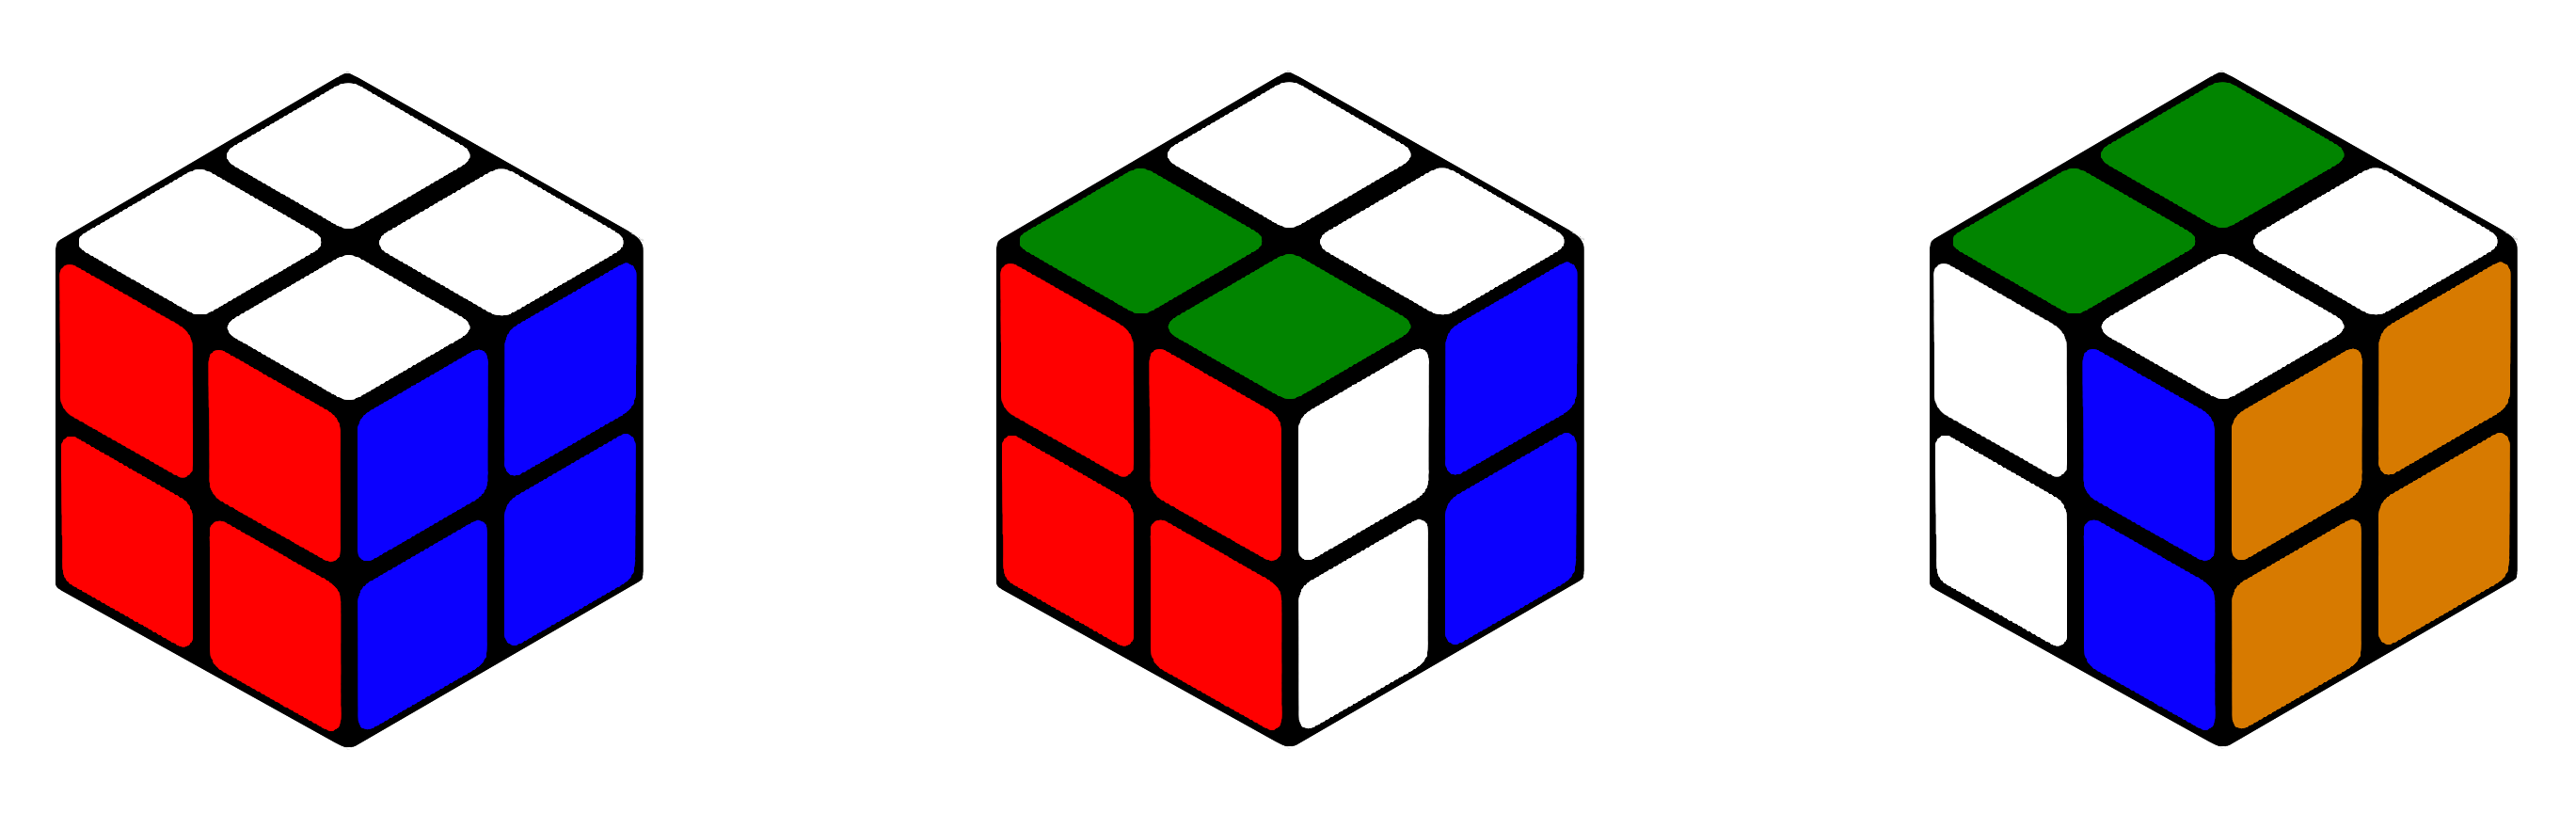
\includegraphics[scale=0.15]{Cube solvedLFzrL.png}
\caption[Cube solved, after move $F$ and after $Z_rL$]{Cube solved (left), after move $F$ (middle) and after $Z_rL$ (right)}
\label{Figure_Cube solved $L$ (left), after move $F$ (middle) and after $Z_rL$ (right)L}
\end{figure}

For $\sim$ to be an equivalence relation, reflexivity, symmetry and transitivity must hold. These properties are shown below for the relation $\sim$.

\begin{description}

\item [Reflexivity] \ \\
For reflexivity, $Z \sim Z$ must hold for all moves. Each move must be in related to itself. The following expressions apply to all $Z$ from $A_Z$ and any cube configuration $C$.
\begin{align*}
Z \sim_R Z & := C \cdot Z = C \cdot WZ
\end{align*}
To show that $Z$ is equivalent to itself, the rotation $W$ is chosen as $N_R$, so that no rotation is performed.
\begin{align*}
Z \sim Z & := C \cdot Z = C \cdot WZ \\
\ & \Leftrightarrow C \cdot Z=C \cdot N_R Z \Leftrightarrow C \cdot Z = C \cdot Z
\end{align*}
For $Z \sim Z$ with $W=N_R$, the move $Z$ is always equivalent to itself, since the same starting configuration produces the same resulting configuration of the cube. Reflexivity, therefore, applies to the relation $\sim$.

\item [Symmetry] \ \\
For symmetry, the following must apply to all $Z_1$ and $Z_2$ from $A_Z$: From $Z_1 \sim Z_2$ follows $Z_2 \sim Z_1$. Below, $C$ is an arbitrary cube configuration.
\begin{align*}
Z_1 \sim Z_2 & \Rightarrow Z_2 \sim Z_1 \\
with \ Z_1 \sim Z_2 & := C \cdot Z_1 = C \cdot WZ_2 \\
\Leftrightarrow C \cdot Z_1 = C \cdot W_1 Z_2 & \Rightarrow C \cdot Z_2 = C \cdot W_2 Z_1
\end{align*}
$Z_2 \sim Z_1$ must hold if $Z_1 \sim Z_2$ holds. Since, $Z_1 \sim Z_2$, the moves $Z_1$ and $Z_2$ are equal with optional rotation.
\begin{description}

\item[Case 1:]
The optional rotation $W$ corresponds to the empty rotation $N_R$. Then the moves $Z_1$ and $Z_2$ lead to the same resulting configuration of the cube and are considered the same:
\begin{alignat*}{2}
& Z_1 \sim Z_2 && \Rightarrow Z_2 \sim Z_1 \textit{ with } W = N_R \\
\Leftrightarrow \ & C \cdot Z_1 = C \cdot N_R Z_2 \ && \Rightarrow C \cdot Z_2 = C \cdot N_R Z_1 \\
\Leftrightarrow \ & C \cdot Z_1 = C \cdot Z_2 && \Rightarrow C \cdot Z_2 = C \cdot Z_1
\end{alignat*}
Consequently, the symmetry holds for $W = N_R$.

\item[Case 2:]
The optional rotation consists of one or more elements from $\{{Z_r}, {Z_l}, {Y_r}, {Y_l}, {X_r}, {X_l}, N_R\}$.
The symmetry holds if $W_2$ is the inverse of $W_1$. The inverse of a rotation is the rotation about the same axis but in the other direction.
The inverse of $W$ is written as $W^{-1}$.
Since the rotations (like the face rotations) are $90^\circ$ rotations, the inverse element of a rotation corresponds to three times the execution of this rotation.
The following applies:
\begin{align*}
\forall \ W \in \{Z_r, Z_l, Y_r, Y_l, X_r, X_l, N_R\} \quad . \quad W^{-1} = WWW = W^3
\end{align*}

Since the rotations were not minimally defined for better clarity, all rotations and the associated inverses are shown in the following table:

\begin{center}
\begin{tabular}{lcccccc}
Rotation $W$ & ${Z_r}$ & ${Z_l}$ & ${Y_r}$ & ${Y_l}$ & ${X_r}$ & ${X_l}$ \\
\hline
Inverse \hspace*{0.1em} $W^{-1}$ & ${Z_l}$ & ${Z_r}$ & ${Y_l}$ & ${Y_r}$ & ${X_l}$ & ${X_r }$ \\
\end{tabular}
\end{center}


If a rotation is composed of several elements from $\{{Z_r}, {Z_l}, {Y_r}, {Y_l}, {X_r}, {X_l}, N_R\}$, the last element must be inverted first.  

So:
\begin{align*}
C \cdot Z_1 = C \cdot W Z_2 & \Rightarrow C \cdot Z_2 = C \cdot W^{-1} Z_1
\end{align*}
This is true because $W^{-1}$ rotates the cube in the opposite direction and the moves result in the same cube configuration again.

\end{description}

And thus, the symmetry holds for $\sim$.



\item [Transitivity] \ \\
It must apply to all moves $Z_1, Z_2$ and $Z_3$ from $A_Z$: From $Z_1 \sim Z_2$ and $Z_2 \sim Z_3$ follows $Z_1 \sim Z_3$. Below, $C$ is an arbitrary cube configuration.
\begin{alignat*}{3}
& Z_1 \sim Z_2  \wedge Z_2 \sim Z_3  \Rightarrow Z_1 \sim Z_3 \\
\Leftrightarrow \ & (C \cdot Z_1 = C \cdot W_1Z_2) \wedge (C \cdot Z_2 = C \cdot W_2Z_3) \ && \Rightarrow (C \cdot Z_1 = C \cdot W_3Z_3)
\end{alignat*}

Since, moves $Z_1$ and $Z_2$ with rotation $W_1$ result in the same cube configuration, and moves $Z_2$ and $Z_3$ also result in the same cube configuration after rotation $W_2$, the relation $\sim$ holds the same for the two moves $Z_1$ and $Z_3$.

Since, the equivalence relation was defined using equality, transitivity applies.

% after rotation $W_3=W_1W_2$, since all necessary rotations have then been carried out:
%\begin{alignat*}{3}
%C \cdot Z_1 = C \cdot W_1Z_2 \ && \wedge C \cdot Z_2 = C \cdot W_2Z_3 \ && \Rightarrow C \cdot Z_1 = C \cdot W_1W_2Z_3
%\end{alignat*}

Transitivity therefore applies to the relation $\sim$.

\end{description}

Since the properties of reflexivity, symmetry and transitivity apply to the relation $\sim$, it is an equivalence relation.

\subsection{Equivalence Classes of Moves}
\label{Section_EquivalenceClassesOfMoves}

 Here, the equivalence classes of the equivalence relation $\sim$ are defined on the set of all moves $A_Z$ and thus, a set is formed that contains these equivalence classes. Each equivalence class is defined as:
\begin{align*}
[Z] := \{ Y \in A_Z \mid Y \sim Z \} \subseteq A_Z
\end{align*}
Accordingly, every equivalence class $[Z]$ contains all moves of the set $A_Z$ that are equivalent to the move $Z$ with the equivalence relation $\sim$. Here, $[Z]$ is a subset of $A_Z$ . All equivalent elements of an equivalence class $[Z]$ are called \textbf{representatives} of this equivalence class. For example, the moves $R$ and $RRRRR$ are representatives of the equivalence class $[R]$, since the moves $R$ and $RRRRR$ are equivalent to $R$ with the equivalence relation $\sim$.

The equality of two moves was defined by the equivalence relation $\sim$. Two moves are considered equivalent if they lead to the same resulting configuration with the same initial configuration with the rotational possibilities of the cube. Therefore, two identical moves $Z_1, Z_2 \in A_Z$ are always representatives of the same equivalence class. Conversely, two moves $Z_1, Z_2 \in A_Z$ that do not lead to the same resulting configuration are representatives of different equivalence classes.\\
The result is that two different equivalence classes do not contain any equivalent moves, since all equivalent moves are in exactly one equivalence class.\\
The set $A_Z / \sim$ will be called $\Gtwo$ from now onwards. It contains the equivalence classes of all cube moves, without containing the same moves or cube rotations twice.
The elements of $\Gtwo$ are all equivalence classes with respect to the equivalence relation $\sim$. The following therefore applies:
\begin{align*}
\Gtwo := \{[Z] \mid Z \in A_Z \}
\end{align*}
$\Gtwo$, therefore contains the equivalence classes of all possible moves of the cube. 

\begin{note}
From now, the third brackets of the equivalence classes in $\Gtwo$ are omitted to simplify the representation of the equations.
\end{note}
Two equivalence classes or their representatives can be linked using the operation $\scriptstyle*$. The moves are then made one after the other (from the left). For the equivalence classes of the moves, the execution of moves is equivalent to the execution of moves defined in section \ref{Section_MovementExecute}.


\subsection{ \Ttwo Rubik's Cubes as a Group}
 \label{Section_CubeAsGroup}

Here, the definition of the group of the \Tthree cube as defined in \cite{JC} is implemented for the group of the \Ttwo cube. The group of the \Ttwo cube is called $\left(\Gtwo, \scriptstyle*\right)$ in the following.


The set $\Gtwo$ consists of the equivalence classes of all possible moves of the cube. Equivalent moves are representatives of the same equivalence class.


The operator $\scriptstyle*$ is defined as a concatenation of two moves. Let $Z_1$ and $Z_2$ be two moves in $\Gtwo$. Then $Z_1 \mathlarger{\scriptstyle*} Z_2$ means that $Z_1$ is executed first and then $Z_2$. $Z_1 \mathlarger{\scriptstyle*} Z_2$ can also be written as $Z_1Z_2$.

We'll now show that  that $\left(\Gtwo, \scriptstyle*\right)$ is a group: 


\begin{description}
\item [Closure Property] \ \\
We've to show $\forall \ Z_1,Z_2 \in \Gtwo \ . \ (Z_1 \mathlarger{\scriptstyle *} Z_2) \in G_{2\times 2\times 2}$. Let $Z_1$ and $Z_2$ be moves and thus elements from $\Gtwo$. Then, $Z_1 \mathlarger{\scriptstyle*} Z_2$ is also an element of $\Gtwo$. The set $\Gtwo$ contains equivalence classes which are defined in section \ref{Section_EquivalenceClassesOfMoves} with the elements from the infinite set of all moves $A_Z$. All elements of the set $A_Z$ are therefore representatives of the equivalence classes in $\Gtwo$. A combination of two moves is also a move from $A_Z$. Thus, $Z_1 \mathlarger{\scriptstyle*} Z_2$ is also representative of an equivalence class in $\Gtwo$. The group $\left(\Gtwo, \mathlarger{\scriptstyle*}\right)$ is therefore closed under the operation $\scriptstyle*$.
 
Also, from section \ref{Section_CardinalityOfG}, the closure of $(\Gtwo, \mathlarger{\scriptstyle*})$ can also be justified differently: In $\Gtwo$, there is a move for every valid cube configuration with which every combination of two valid moves leads to a valid cube configuration. Therefore, the group $\left(\Gtwo, \mathlarger{\scriptstyle*}\right)$ is closed.


\item [Associativity] \ \\
We've to show $\forall \ Z_1,Z_2,Z_3 \in \Gtwo \ . \ (Z_1 \mathlarger{\scriptstyle*} Z_2) \mathlarger{\scriptstyle*} Z_3 = Z_1 \mathlarger{\scriptstyle*} (Z_2 \mathlarger{\scriptstyle*} Z_3)$

To show associativity, we denote a cubie in the cubie by $s$. When making a move $Z$, $Z(s)$ is now written to get the new position of the cubie. The positions are 3-letter abbreviations consisting of $u, d, r, l, f, b$ [Section \ref{Name}]

When considering $Z_1 \mathlarger{\scriptstyle*} Z_2 $, $Z_1$ is executed first and then $Z_2$. $Z_1$ moves the cubie $s$ to the position $Z_1(s)$. The move $Z_2$ then moves the cubie to the position $Z_2(Z_1(s))$. Consequently, $Z_1 \mathlarger{\scriptstyle*} Z_2 = Z_2(Z_1(s))$.


Now, we've to show $(Z_1 \mathlarger{\scriptstyle*} Z_2) \mathlarger{\scriptstyle*} Z_3 = Z_1 \mathlarger{\scriptstyle*} (Z_2 \mathlarger{\scriptstyle*} Z_3)$. Our target is to transform both $(Z_1 \mathlarger{\scriptstyle*} Z_2) \mathlarger{\scriptstyle*} Z_3$ and $Z_1 \mathlarger{\scriptstyle*} (Z_2 \mathlarger{\scriptstyle*} Z_3)$ c to $Z_3(Z_2(Z_1(s))$:
\begin{align*}
& (Z_1 \mathlarger{\scriptstyle*} Z_2) \mathlarger{\scriptstyle*} Z_3 \\
\Leftrightarrow (&(Z_1 \mathlarger{\scriptstyle*} Z_2) \mathlarger{\scriptstyle*} Z_3)(s) \\
= & Z_3(Z_1 \mathlarger{\scriptstyle*} Z_2)(s)) \\
= & Z_3(Z_2(Z_1(s)))
\\
\\
&Z_1 \mathlarger{\scriptstyle*} (Z_2 \mathlarger{\scriptstyle*} Z_3) \\
\Leftrightarrow (&Z_1 \mathlarger{\scriptstyle*} (Z_2 \mathlarger{\scriptstyle*} Z_3))(s) \\
= (&Z_2 \mathlarger{\scriptstyle*} Z_3)(Z_1(s)) \\
= \ \ & Z_3(Z_2(Z_1(s)))
\end{align*}
Thus, $(\Gtwo, \mathlarger{\scriptstyle*})$ is associative.


\item [Existence of  Identity Element $\boldsymbol{N}$] \ \\

We've to show that $\exists \ N \in \Gtwo \ \forall \ Z \in \Gtwo \ . \ N \mathlarger{\scriptstyle*} Z = Z \mathlarger{\scriptstyle*} N = Z$


The identity element $N$ must be an element from $\Gtwo$ such $\forall$ moves $Z \in \Gtwo$ the following must hold:
\begin{align*}
N \mathlarger{\scriptstyle*} Z = Z \mathlarger{\scriptstyle*} N = Z
\end{align*}
The identity element of the group $(\Gtwo, \mathlarger{\scriptstyle*})$ is the empty move. None of the faces of the cube are rotated. If a move $Z$ is made and then the move $N$ is made, it means \textit{ $Z$ executed first and then nothing}, which is the same as \textit{ $Z$}.

So, executing $N$ does not change the cube configuration. The permutation function for the identity element is then $\sigma_N=1$ and the transition function $\gamma_N$ of the vector $x$ is $\gamma_N(x)=x$. The proof of this can be found in appendix \ref{Appendix_AlignmentFunctions}.

For the identity element, the following must apply to each cube configuration $C$:
\begin{align*}
C \cdot N = C
\end{align*}

This applies, for example rotating a single layer four times. The configuration $C$ is then back in the initial configuration. The following statement was proven in Appendix \ref{Appendix_AlignmentFunctions}. If $(\sigma, x)$ is any cube configuration, then $\forall \ Z \in \{U, D, R, L, F, B\} $
\begin{align*}
(\sigma, x) \cdot Z^4 = (\sigma, x)  
\end{align*}
holds. \\
For any move $Z$ from $\Gtwo$, $Z^0=N$ also applies, since the cube configuration remains unchanged if a move is executed zero times.

The identity element $N$ of $(\Gtwo, \mathlarger{\scriptstyle*})$ is therefore the equivalence class of the empty move.


\item [Existence of an Inverse Element $\boldsymbol{Z^{-1}}$] \ \\
We've to show that $\forall \ Z \in \Gtwo \ \exists \ Z^{-1} \in \Gtwo \ . \ Z \mathlarger{\scriptstyle*} Z^{-1} = Z^{-1} \mathlarger{\scriptstyle*} Z = N$


Each move $Z$ transforms one cube configuration into a resulting configuration.
This is understood by a permutation function $\sigma$ and a transition function $\gamma$ for the vector $x$.
So, if we see the cube, then we can also rotate the individual layers counterclockwise, thus inverting a layer rotation. A face rotation of $90^\circ$ counterclockwise is equivalent to a face rotation of $270^\circ$ clockwise. The functions $\sigma$ and $\gamma$ are the same.
The inverses of the individual face rotations are therefore defined as :
\begin{align*}
\forall \ Z \in \{U, D, R, L, F, B\} \ . \ Z^{-1} = ZZZ = Z^3
\end{align*}
If we want to invert a move that consists of several basic moves, the last element must be inverted first. For a move $Y$ of length $n$, the elements of the entire move are inverted from behind. Here $n \in \mathbb {N}$ and $Z_i$ represents all sub-moves $Z_1$ - $Z_n$ that make up the move $Y$.
\begin{align*}
\forall \ Y \in \Gtwo, Y & = (Z_1 \mathlarger{\scriptstyle*} Z_2 \mathlarger{\scriptstyle*} ... \mathlarger{\scriptstyle*} Z_n), Z_{i} \in \{U, D, R, L, F, B\} \ . \ \\
Y^{-1} & = {Z_n}^{-1} \mathlarger{\scriptstyle*} {Z_{n-1}}^{-1} \mathlarger{\scriptstyle*} ... \mathlarger{\scriptstyle*} {Z_1}^{-1}
\end{align*}
This can be transformed using the above definition of $Z^{-1}$ with $Z \in \{U, D, R, L, F, B\} $ as follows:
\begin{align*}
Y^{-1} & = {Z_n}^{-1} \mathlarger{\scriptstyle*} {Z_{n-1}}^{-1} \mathlarger{\scriptstyle*} ... \mathlarger{\scriptstyle*} {Z_1}^{-1} \\
& = Z_nZ_nZ_n \mathlarger{\scriptstyle*} Z_{n-1}Z_{n-1}Z_{n-1} \mathlarger{\scriptstyle*} ... \mathlarger{\scriptstyle*} Z_1Z_1Z_1 \\
& = {Z_n}^3 \mathlarger{\scriptstyle*} {Z_{n-1}}^3 \mathlarger{\scriptstyle*} ... \mathlarger{\scriptstyle*} {Z_1}^3 \\
& = {Z_n}^3{Z_{n-1}}^3 ... {Z_1}^3 \\
\end{align*}
These expressions define the inverse elements for each move from $\Gtwo$.

\end{description}
Thus, $(\Gtwo, \mathlarger{\scriptstyle*})$ is a group. 

$(\Gtwo, \mathlarger{\scriptstyle*})$ is not an abelian group because, for example, a clockwise rotation of the right face ($R$) and a clockwise rotation of the front face ($F$) in reverse order have different results. This example is shown in Figure \ref{Figure_CubeAfterFRandRF}.
\begin{figure}[H]
\centering
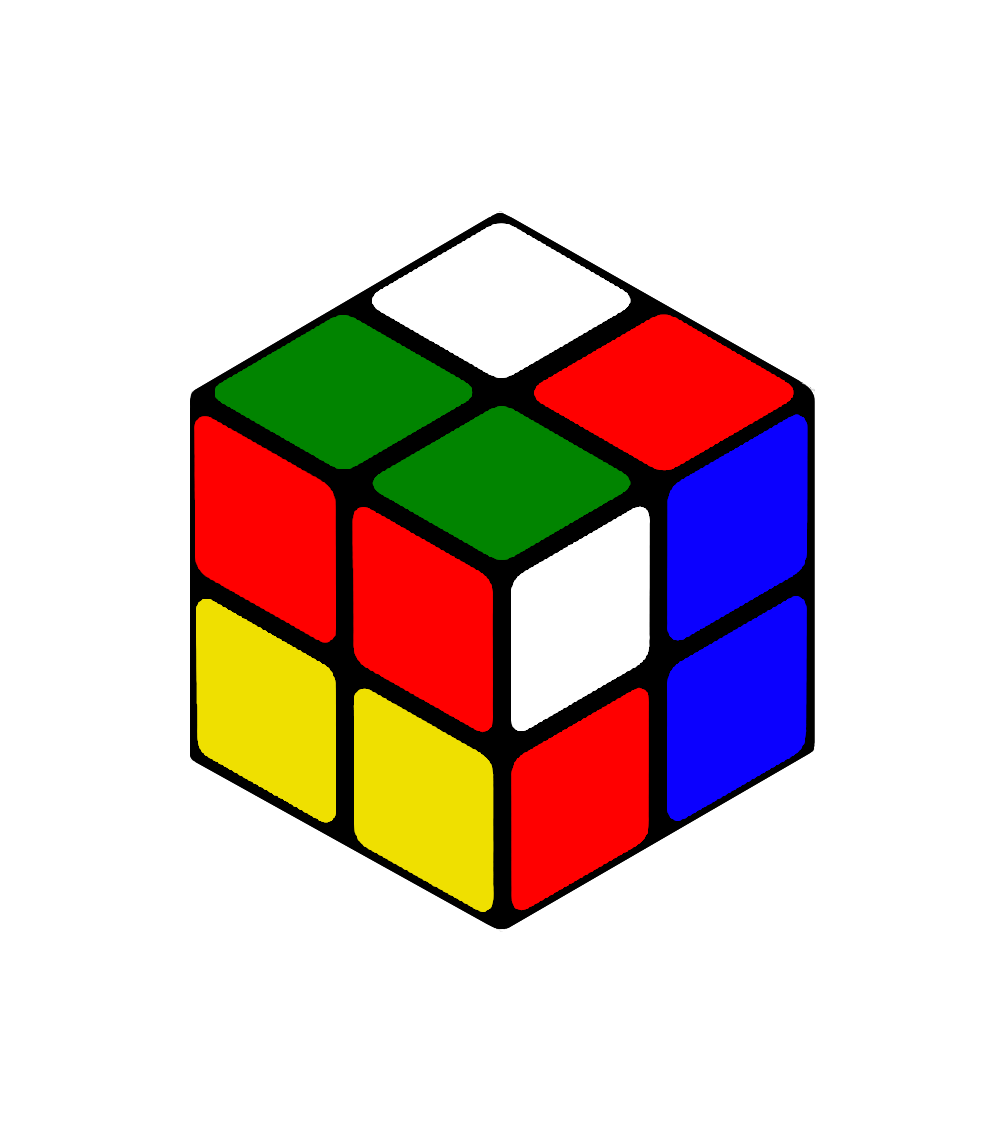
\includegraphics[scale=0.1]{RF.png}
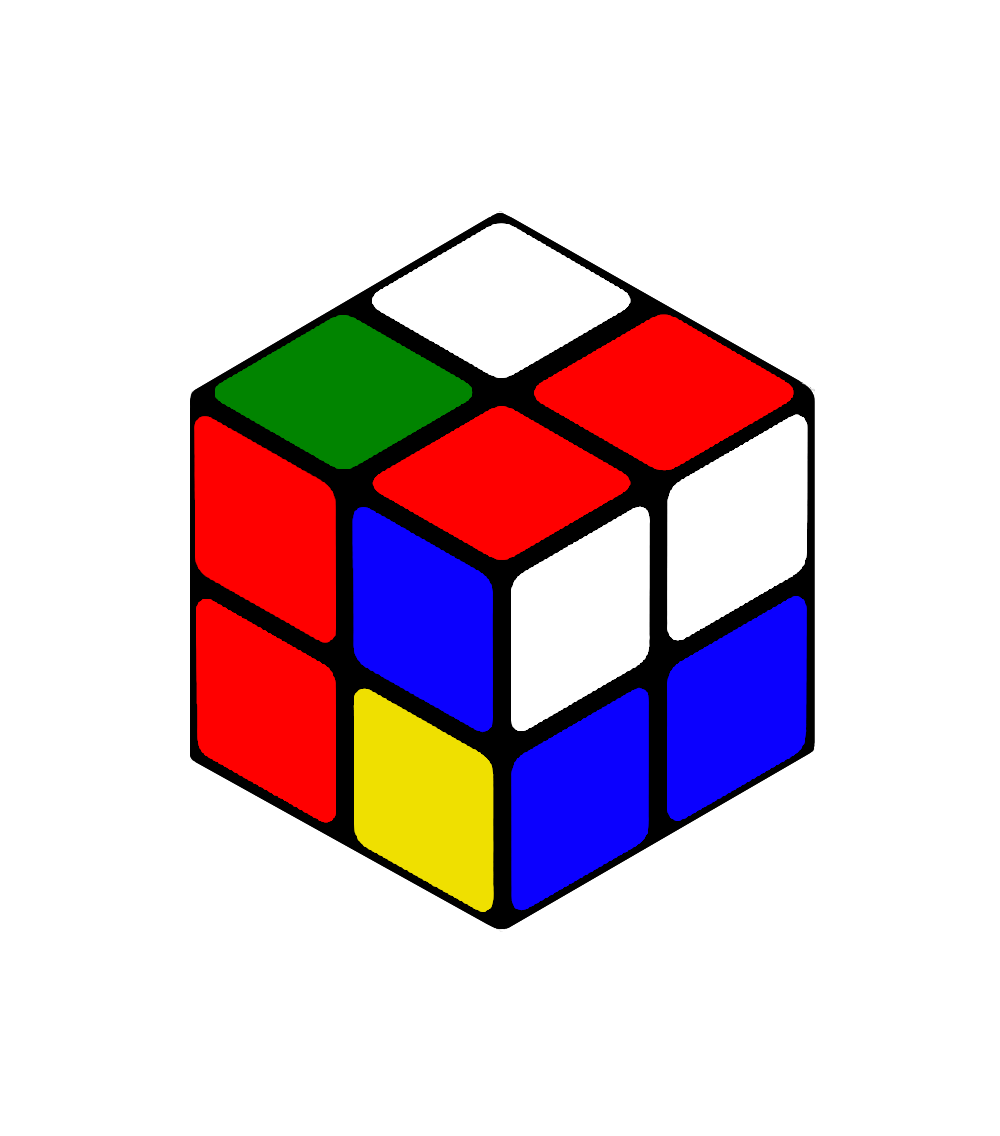
\includegraphics[scale=0.1]{FR.png}
\caption[Cube after moves $FR$ (left) and $RF$ (right)]{Cube after moves $FR$ (left) and $RF$ (right)}
\label{Figure_CubeAfterFRandRF}
\end{figure}
Furthermore, solving the cube would be trivial if commutativity holds. \cite{TD} The order of the rotated layers would then be irrelevant and only the number would've to be taken into account.
Accordingly, $\forall \ Z_1, Z_2 \in \Gtwo$ does not apply. $Z_1 \mathlarger{\scriptstyle*} Z_2 = Z_2 \mathlarger{\scriptstyle*} Z_1$ and the $\mathlarger{\scriptstyle*}$ operation of the group is, therefore, not commutative.

\subsection{Moves as Group Operation}
Here, I'll introduce \textbf{group operation: move} that maps a cube configuration to a new cube configuration by making a move. %In group operations, the elements of a group affect a lot. In this case, the moves of the cube affect the configuration of the cube. It is the right operation because the elements of the group operate on the elements of the set from the right. The right operation was defined. 

$\Gtwo$ is the set of the group $\left(\Gtwo, \scriptstyle*\right)$ and $M_C$ is the set of all configurations. The $\scriptstyle*$ operator of the group operation is defined as follows:
\begin{align*}
\cdot: M_C \times \Gtwo \rightarrow M_C
\end{align*}
If an arbitrary configuration $C=(\sigma, x)$ from the set of configurations $M_C$ is transferred into a new configuration by executing a move $Z \in \Gtwo$, then this resulting configuration is called $(C \cdot Z)  \in M_C$.
The following two properties must apply to the legal operation:

\begin{description}
\item [$\boldsymbol{C \cdot N = C}$ for all $\boldsymbol{C \in M_C}$ and the identity element $\boldsymbol{N \in \Gtwo}$]
\ \\
When the empty move $N$ is made, the configuration of the cube is not changed. The identity move transfers the configuration with $\sigma_N=1$ and $\gamma_N(x)=x$. Both the permutation function $\sigma$ and the vector $x$ remain unchanged when the move $N$ is executed. \newpage Therefore:
\begin{align*}
 C \cdot N
\Leftrightarrow \ \ & (\sigma, x) \cdot N \\
= \ \ & (\sigma_N \cdot \sigma, \gamma_N(x)) \\
= \ \ & (\sigma, x) \\
= \ \ & C
\end{align*}

\item [$\boldsymbol{C \cdot (Z_1 \mathlarger{\scriptstyle*} Z_2) = (C \cdot Z_1) \cdot Z_2}$ for all $\boldsymbol{Z_1, Z_2 \in \Gtwo}$ and $\boldsymbol{C \in M_C}$]
\ \\
Let $C$ be a configuration of the cube. If the move $Z_1 \in \Gtwo$ is executed starting from the configuration $C$, the new configuration of the cube is $C \cdot Z_1$. If another move $Z_2 \in \Gtwo$ is made, the new configuration of the cube is $(C \cdot Z_1) \cdot Z_2$.
It was therefore started with configuration $C$ and the moves $Z_1$ and $Z_2$ were executed. This can be transformed into the following:
\begin{align*}
& (C \cdot Z_1) \cdot Z_2 \\
\Leftrightarrow \ & C \cdot Z_1Z_2 \\
\Leftrightarrow \ & C \cdot (Z_1 \mathlarger{\scriptstyle*} Z_2)
\end{align*}
The new configuration can therefore also be written as $C \cdot (Z_1 \mathlarger{\scriptstyle*} Z_2)$ and therefore $(C \cdot Z_1) \cdot Z_2 = C \cdot (Z_1 \mathlarger{\scriptstyle*} Z_2)$.
\end{description}
\nopagebreak
Since, both properties apply, it is a group operation. 

\subsection{Order of Permutations}

\label{Section_OrderPermutations}
In the sections \ref{Section_EqualityOfmoves} and \ref{Section_MaxNumberRotations}, for any cube configuration $C$, it was shown that:
\begin{align*}
\forall \ Z \in \{ U, D, R, L, F, B \}, n \in \mathbb{N} \ . \ C \cdot Z^n=C \cdot Z^{n \hspace*{-0.5em} \mod 4}
\end{align*}
\vspace*{-3em}
\begin{align*}
\forall \ T \in \{{Z_r}, {Z_l}, {Y_r}, {Y_l}, {X_r}, {X_l}, I_R \}, n \in \mathbb{N} \ . \ C \cdot T^n=C \cdot T^{n \hspace*{-0.5em} \mod 4}
\end{align*}
This means that if a single-element face rotation is performed four times in a row, all of the cube's pieces will return to their previous positions. Therefore, the basic moves $U, D, R, L, F, B$ and the rotations $X_r, X_l, Y_r, Y_l, Z_L, Z_r$ are called permutations of order 4.

Not only the moves $U, D, R, L, F, B$ return to their initial state after repeating. All other moves, when performed repeatedly, bring the cube back to the starting position that the cube had before the move was made \cite{TD}. Depending on the move, different numbers of repetitions are required.


It should be noted that in this section, I've only discussed the ordering of the permutations. If we transfer this to the cube configuration, only the cubie position $\sigma$ is taken into account. The order of the permutations is therefore the number of turns/twists required for all cubies to return to their original position. However, the orientation of the cubies is not taken into account here. The order in relation to the complete cube configuration is described in section \ref{Section_Ordermoves} as \textit{Order of Moves}. In this section, the order of the permutation is defined and described using an example. In addition, the cycle structure is represented through Cayley Graph and an algorithm for calculating the permutation order is then introduced.


\begin{example}

For example, the permutation of the move $(LLFF)$ has order 3, since the cube is back in the starting position after repeating $(LLFF)$ three times. Then $(LLFF)^3 = N$.
Other example moves with an indication of the order are: ${R^4= N}$ (order 4) or ${(RRFF)^3 = N}$ (order 3).
\end{example}


The examples mentioned can be tried out manually on a \Ttwo cube.
\begin{note}
It must be noted that the order of the permutations differs from the order of the moves.
\end{note}

Now, we'll define the order of permutation. 
\begin{definition}
    

  
The \textbf{order of a permutation} for any $(\sigma, x)$ cube configuration is defined as: 
\begin{align*}
\forall \ Z \in \Gtwo \ \exists \ n \in \mathbb{N} \ . \ (\sigma, x) \cdot Z^n = (\sigma, x')
\end{align*}
Therefore, for any move $Z$, there is $n \in \mathbb{N}$, which is the order of the permutation of the move. If this move $Z$ is executed $n$ times, the permutation function $\sigma$ returns to its initial state. Here, the vector $x$ is not taken into account.
\end{definition}
\begin{note}
    The order of a permutation is all about the cubie positions and not the cubie orientations.
\end{note}
\begin{example}
    
For example, the move $LF$ has order $15$, but the permutation of the cubies has order $5$. After five repetitions of $LF$, all cubies are back in their starting position (on the left in Figure \ref{Figure_LF_5_15}, starting from the starting configuration). After $15$ repetitions, the cube is back in the same configuration as before the move (right in Figure \ref{Figure_LF_5_15}).

\begin{figure}[H]
\centering
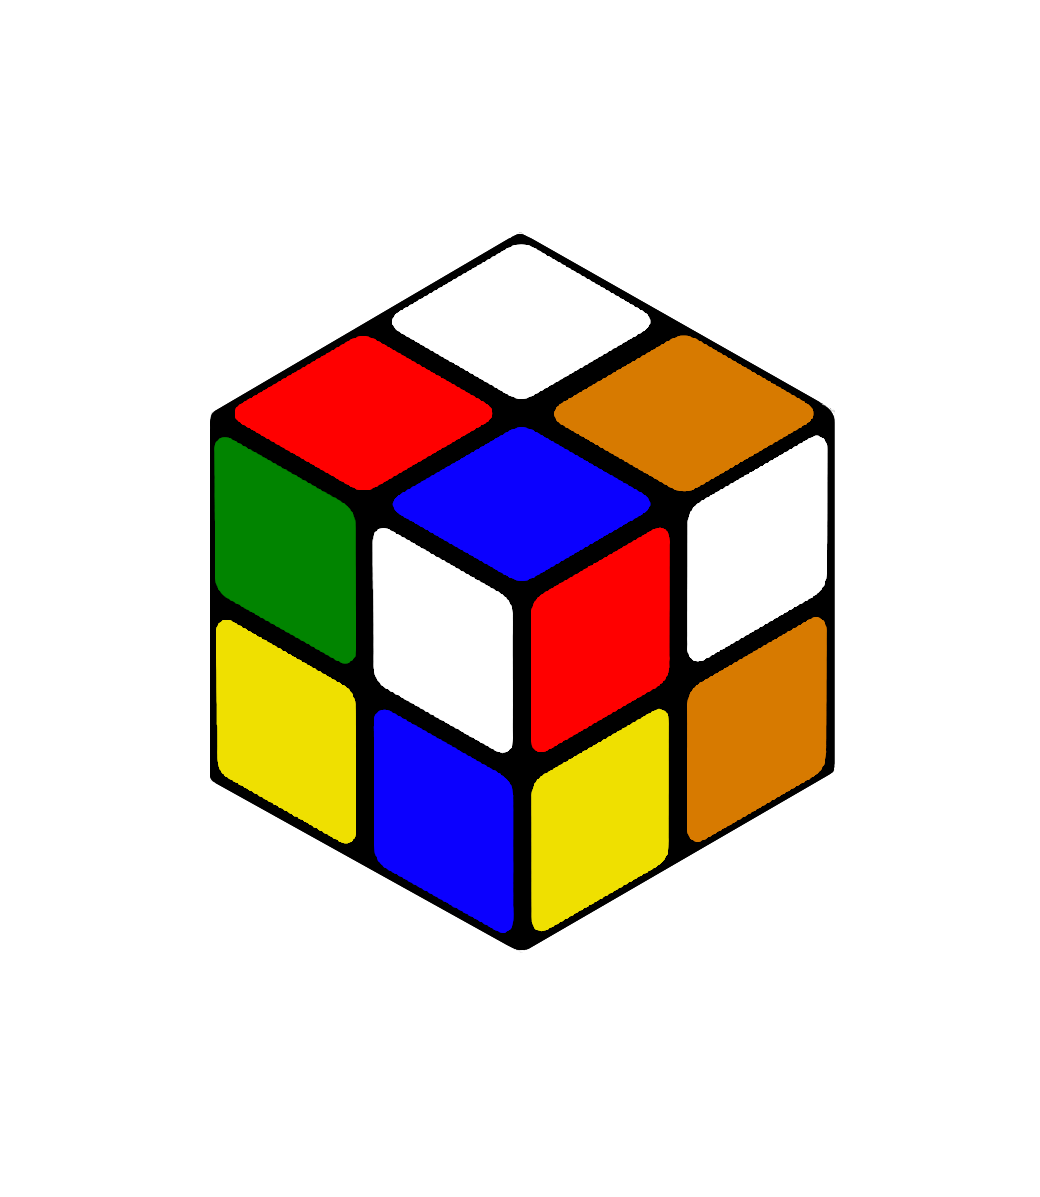
\includegraphics[scale=0.15]{LLFF_5.png}
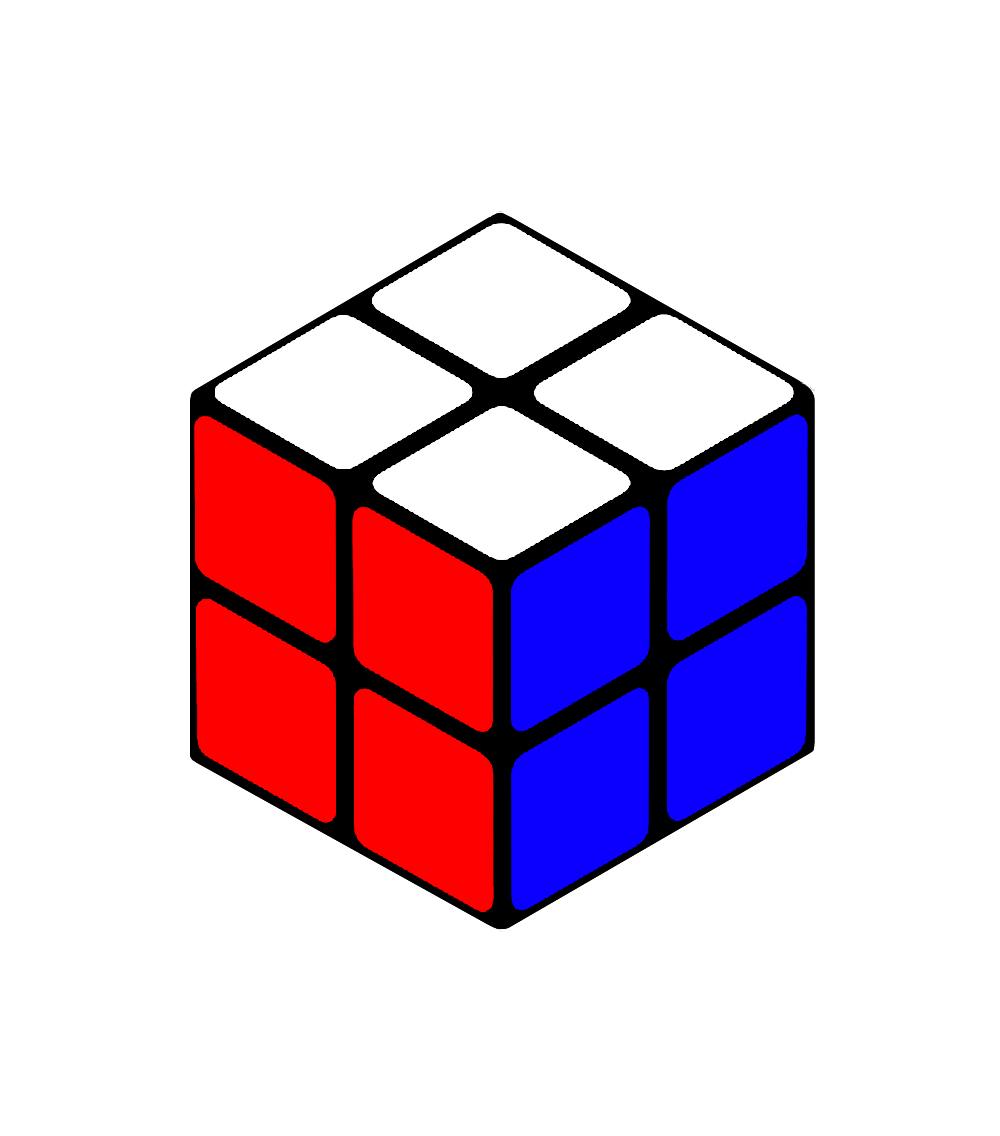
\includegraphics[scale=0.15]{2x2solved.png}
\caption{Executing $LF$ five times (left) and 15 times (right)}
\label{Figure_LF_5_15}
\end{figure}

On the left in Figure \ref{Figure_LF_5_15}, we can see that all cube pieces are in their respective starting positions, but not correctly aligned. If the move $(LF)^5$ is applied to the starting configuration $(1,0)$, this resulting configuration is obtained:
\begin{align*}
(1,0) \cdot (LF)^5 = (1, (1,0,1,1,1,0,1,1))
\end{align*}
The cube is not solved after five repetitions of $LF$ because the orientation of the cubies is changed -- the vector $x$ is not 0. The order of the permutation of $LF$ is 5 because the function $\sigma$ is 1 after executing five times. However, the order of $LF$'s move is 15, because only then does the cube return to its original configuration. Thus, after executing $(LF)^{15}$, the cube configuration is $(1,0)$ again at the starting state:
\begin{align*}
(1,0) \cdot (LF)^{15} = (1,0)
\end{align*}
This then also applies to any other configuration $(\sigma, x)$ after executing the move $(LF)^{15}$:
\begin{align*}
(\sigma, x) \cdot (LF)^{15} = (\sigma, x)
\end{align*}
\end{example}


\subsubsection*{Cycle structure}
\label{section_cycle structure}

The order of a permutation can be determined based on its cycle structure. 

For example, the permutation function $\sigma_U =\ ( \ \textit{ulf} \ \textit{ulb} \ \textit{urb} \ \textit{urf} \ ) $ consists of the move $U$ (a rotation of the upper layer by $90 ^\circ$ clockwise) from exactly one four-element cycle.
If the move $U$ is executed four times, the cubies are back in their previous position. The following table shows running the permutation $\sigma_U$ four times.
\begin{center}
\begin{tabular}{ccccc}
\toprule
\textbf{Execution No.} & \textbf{ulf} & \textbf{ulb} & \textbf{urb} & \textbf{urf} \\
\midrule
1 & ulb & urb & urf & ulf \\

2 & urb & urf & ulf & ulb \\

3 & urf & ulf & ulb & urb \\

4 & ulf & ulb & urb & urf \\
\bottomrule
\end{tabular}
\end{center}

The fourth row of the table has the same arrangement of cubies as the top row (before executing $U$).
Thus, the permutation of the described face rotation $U$ has order 4, since $\sigma_U$ leads back to the original permutation after four repetitions. This also applies to the other one-element moves ($D, F, B, L, R$).
For any permutation of a move $Z$ that consists of only one $n$-element cycle, the order of the permutation is $n$, where $(\sigma, x)$ is an arbitrary cube configuration:
\begin{align*}
\forall \, Z \in \Gtwo \ \text{with} \ \sigma_Z=(i_1 \ i_2 \ ... \ i_n) \ \exists \, n \in \mathbb{N} \ . \ (\sigma, x) \cdot Z^n= (\sigma, x')
\end{align*}
If the move $Z$ is executed multiple times, the initial state of the permutations is reached \cite{TD} after every $n^\text{th}$ repetition.
It, therefore, also applies:
\begin{align*}
\forall \, Z \in \Gtwo \ \textit{with} \ Z=(i_1 \ i_2 \ ... \ i_n), \, k \in \mathbb{N} \ \exists \, n \in \mathbb {N} \ . \ {(\sigma, x) \cdot Z^{k*n}=(\sigma, x') }
\end{align*}
Even with more complex permutations of moves that consist of more than one cycle, the order can be determined based on the cycle structure. To do this, the \textit{least common multiple (lcm)} of all cycle lengths must be determined. \cite{TD}
\newpage
 
For better clarity, the cycles of all moves are shown in Figure \ref{Figure_GraphAllerPermutations}. The figure makes it easier to read the cycles when multiple face rotations are combined in one move.

\begin{figure}[H]
\centering
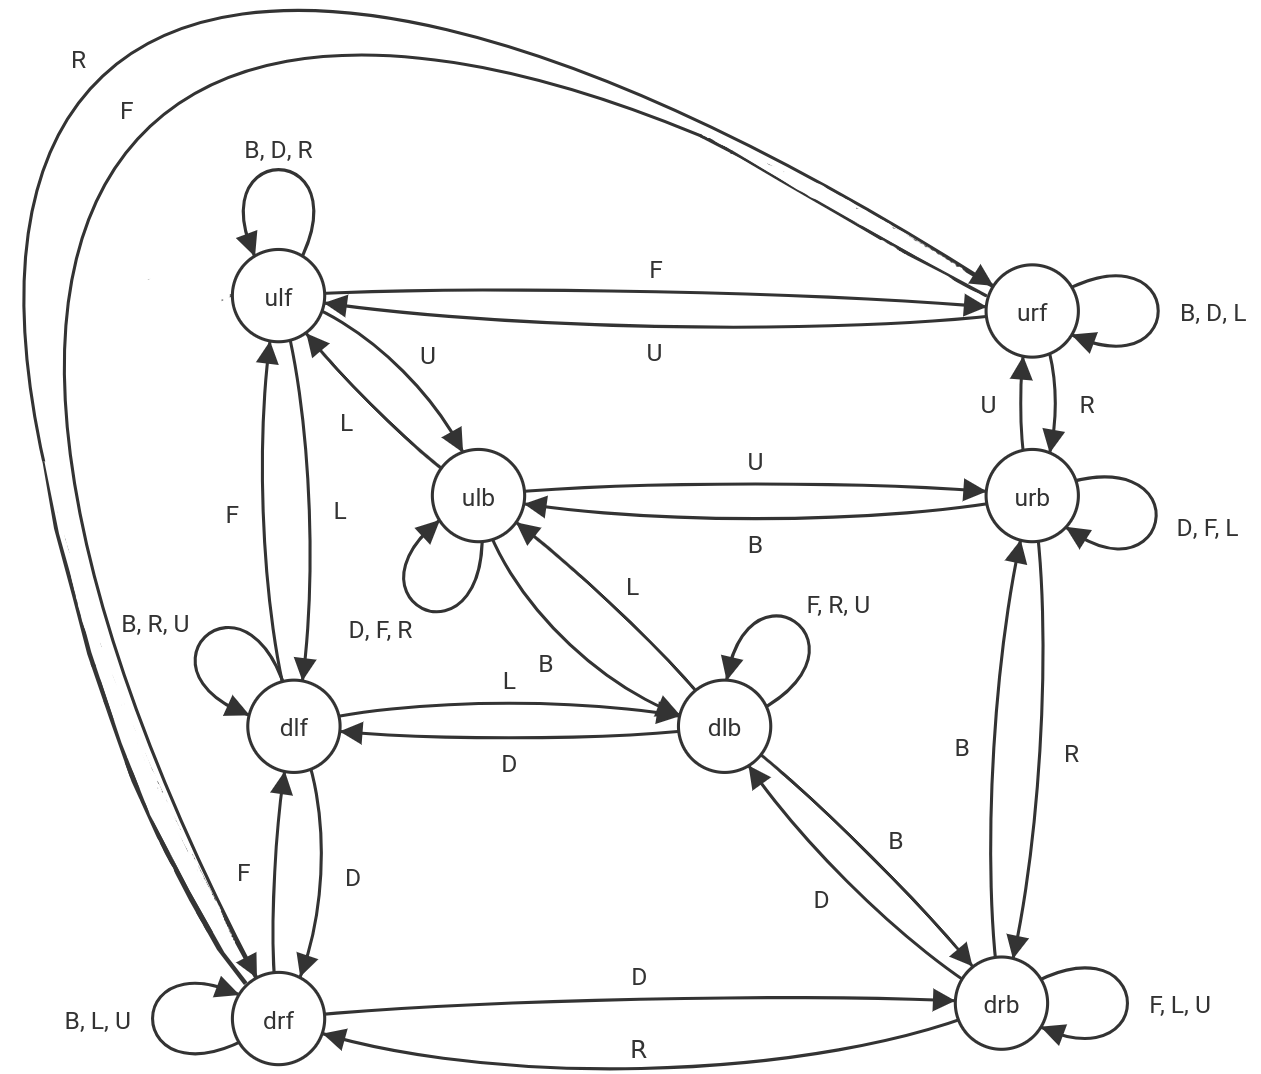
\includegraphics[scale=0.3]{Cayley graph of all permutations.png}
\caption[Graph of all move permutations]{Cayley Graph of Permutation of all moves}
\label{Figure_GraphAllerPermutations}
\end{figure}

Using the graph or the permutation functions $\sigma$, the cycle structure of the permutations for the example move $LLFF$ can now be represented.
To do this, a table is created that maps each position to its new position. The move $LLFF$ is composed of the moves $L$ and $F$.

\begin{center}
\begin{tabular}{ccccccccc}
\toprule
\textbf{Move} & \textbf{ulb} & \textbf{urb} & \textbf{ulf} & \textbf{urf} & \textbf{dlb} & \textbf{drb} & \textbf{dlf} & \textbf{drf} \\
\midrule

L & ulf & \textcolor{gray}{urb} & dlf & \textcolor{gray}{urf} & ulb & \textcolor{gray}{drb} & dlb & \textcolor{gray}{drf} \\

L & dlf & \textcolor{gray}{urb} & dlb & \textcolor{gray}{urf} & ulf & \textcolor{gray}{drb} & ulb & \textcolor{gray}{drf} \\

F & ulf & \textcolor{gray}{urb} & \textcolor{gray}{dlb} & drf & urf & \textcolor{gray}{drb} & \textcolor{gray}{ulb} & dlf \\

F & urf & \textcolor{gray}{urb} & \textcolor{gray}{dlb} & dlf & drf & \textcolor{gray}{drb} & \textcolor{gray}{ulb} & ulf \\
\bottomrule
\end{tabular}
\end{center}
The gray entries remain unchanged with the respective layer rotation.\newpage
The cycles of the move $LLFF$ are shown in Figure \ref{CycleOfLLFF}. There you can see that $LLFF$ consists of two one-element and two three-element cycles.
\begin{figure}[H]
\centering
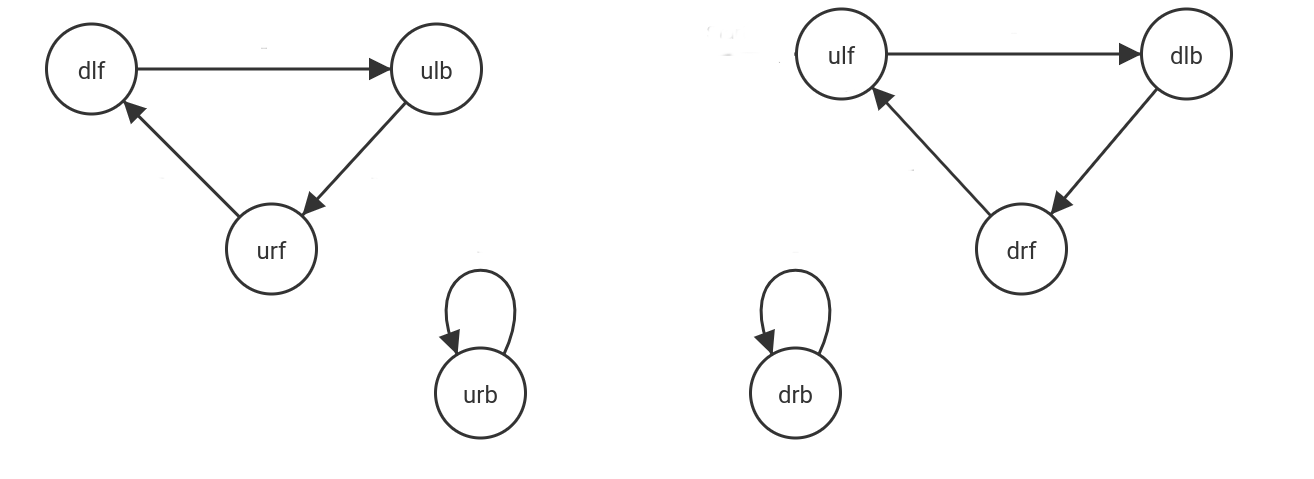
\includegraphics[scale=0.3]{cycle_LLFF.png}
\caption[Cycle of move $LLFF$]{Cycle of move $LLFF$}
\label{CycleOfLLFF}
\end{figure}
In the cyclic notation, the move $LLFF$ is therefore written as $\sigma_{LLFF}=( \ \textit{dlf} \ \textit{ulb} \ \textit{urf}\ )(\ \textit{ulf} \ \textit{ dlb} \ \textit{drf} \ )$ is written.
Since there are two cycles of length three, all cubies are back in their original position after three moves:
\begin{align*}
kgV(3,3,1,1)=3
\end{align*}
So, the permutation of the move $LLFF$ has order $3$.
It can also be seen that six of the eight cubies are moved on the move $LLFF$. The other two (\textit{urb} and \textit{drb}) remain unchanged. This can be seen in the representation of the cycles (Figure \ref{CycleOfLLFF}).
In the example move $LLFF$, after executing the move $3$ times, not only the position of the cubies is correct, but also the alignment. So, the \textit{order of the moves} is also 3. 

\subsubsection*{Algorithm}

These findings result in the following algorithm for determining the order of a permutation. A move $Z$ is passed as an input parameter. The return is the permutation order of the move $Z$.\newpage

\begin{minipage}[H]{0.14\textwidth}
      $\ $
\end{minipage}
\begin{minipage}[H]{0.72\textwidth}
\begin{algorithm}[H]
\LinesNumbered
\DontPrintSemicolon
\SetNlSty{textbf}{}{\ }
\SetAlgoNlRelativeSize{0}
\KwData{Move $Z$}
\KwResult{\textit{kgVList} is the Order of the Permutation}
\BlankLine
 \textit{perm} $\leftarrow$ Permutation Function of Move $Z$\;

  \textit{list} $\leftarrow$ Empty List \;
  
  \textit{kgVList} $\leftarrow$ 0 \;

  \textit{z} $\leftarrow$ Number of Cycles of $perm$ \; 

 \While{\textit{z} $> 0$}{
 
  \textit{cycleLength} $\leftarrow$ Cycle Length of cycle $z$ \;
  
  \textit{list} $\leftarrow$ \textit{cycleLength} add \;
  
  \textit{z} $\leftarrow$ \textit{ z}$-1$ \;
 }
  \textit{kgVList} $\leftarrow$ \textit{kgV} of elements from  \textit{list} calculate \;

 return \textit{kgVList} \;

\caption{Determine the Order of a Permutation} 
\label{Algorithm_OrderPermutation}
\end{algorithm}
\end{minipage}
\begin{minipage}[H]{0.14\textwidth}
      $\ $
\end{minipage}

In line 1, the permutation function of the move is assigned to the variable \textit{perm} and in line 2 an empty list is initialized to store the lengths of the individual cycles. Then in line 3 the variable \textit{kgVList} is initialized with 0. In line 4, the number of cycles is read and stored in the variable $z$. A \textit{while} loop is then executed $z$ times. In each pass, the length of one of the $z$ cycles is read and added to the list (lines 6-7). Additionally, $z$ is decremented (line 8). After all cycle lengths are stored in \textit{list}, the \textit{least common multiple} of the list elements is calculated in line 9 and assigned to the variable \textit{kgVList}. This is the order of the permutation and, therefore, \textit{kgVList} is returned in line 10.

The order of the permutation is needed to calculate the order of moves. This is described in the following section and an algorithm for calculating it is also discussed.
\subsection{Order of Moves}
\label{Section_Ordermoves}
Here, we'll see that the cube returns to its original position when any move $Z \in \Gtwo$ is repeatedly applied to the cube. This is shown in the following formula, where $C$ is any cube configuration.
\begin{align*}
\forall \ Z \in \Gtwo \ \exists \ n \in \mathbb{N} \ . \ C \cdot Z^n = C
\end{align*} \nopagebreak An algorithm for calculating the order of moves is also described.
\subsubsection*{Proof}

The following proof is based on a proof from \cite{TD}.

Each time a move is repeated, the cubies in the cube are rearranged and aligned.\\
Since there are a finite number of cube configurations, a cube configuration gets repeated if a move is made often enough.
The number of valid cube configurations is very large, but finite ($3 , 674 , 160$). Accordingly, a configuration gets repeated if the move is made more often than there are possible cube configurations. The number of valid cube configurations is calculated in section \ref{Chapter_ValidConfigurations}.

So, this means: With any move $Z \in \Gtwo$ that is applied to any configuration $C$, a cube configuration is repeated after repeated execution. If the repeated configuration $C'$ occurs first after $n \in \mathbb{N}$ repetitions of move $Z$ and the second time after $m \in \mathbb{N}$ repetitions, then:
\begin{align*}
C' = C \cdot Z^n& = C \cdot Z^m \textit{ with } 0<n<m
\end{align*}
Since $n$ and $m$ represent the first occurrence of a repeating configuration, then:
\begin{align*}
C \cdot Z^{n-1} \neq C \cdot Z^{m-1}
\end{align*}

If the move $Z$ is applied $n$ times or $m$ times to the same initial configuration $C$, the same resulting configuration $C'$ is achieved.
If the move $Z^{-1}$ is, then, applied to this configuration $C'$, the resulting configuration $C'''$ is  same again. It is irrelevant whether it was previously executed $n$ times or $m$ times $Z$. Starting from the same initial configuration, the same resulting configuration is achieved when the same move is made. Accordingly:
\begin{alignat*}{2}
\ &(C \cdot Z^n) \cdot Z^{-1} && = (C \cdot Z^m) \cdot Z^{-1} \\
\Leftrightarrow \ & C' \cdot Z^{-1} && = C' \cdot Z^{-1} \\
\Leftrightarrow \ & C'' && = C ''
\end{alignat*}
Applying $Z^{-1}$ to the configuration $C'$ will undo the last execution of $Z$ because $Z^{-1}$ is the inverse of the move $Z$. If the move $Z$ is made $n$ times and then $Z^{-1}$ is made, it is the same as making $Z$ , $n-1$ times. Consequently:
\begin{align*}
(C \cdot Z^n) \cdot Z^{-1}=C \cdot (Z^n \mathlarger{\scriptstyle*}  Z^{-1})=C \cdot Z^{n-1}
\end{align*}
The following also applies:
\begin{alignat*}{2}
 & (C \cdot Z^n) \cdot Z^{-1}  = (C \cdot Z^m) \cdot Z^{-1} \\
\Leftrightarrow \ & C \cdot Z^{n-1}  = C \cdot Z^{m-1}
\end{alignat*}
However, this then contradicts the assumption that $m$ is the smallest value for repeating the configuration. In this case, $n-1$ or $m-1$ is the smallest number of executions for a repeating configuration:
\begin{alignat*}{2}
 & (C \cdot Z^n) \cdot Z^{-1}  = (C \cdot Z^m) \cdot Z^{-1} \\
\Leftrightarrow \ & C \cdot Z^{n-1}  = C \cdot Z^{m-1} \\
\Leftrightarrow \ & C''  = C''
\end{alignat*}
Therefore, it must be $n=0$ must for $m$ to represent the first repetition of a position.

This means that if a move is repeatedly applied to a cube, the cubies return to their original position.

\subsubsection*{Algorithm}

It has already been shown that a cube configuration repeats itself when any move is applied repeatedly. 
\begin{definition}
    The number of repetitions of a move until the cube returns to its original configuration is called the \textbf{order of a move}.
\end{definition}
An algorithm is now designed to calculate this, which is presented as pseudo-code. The algorithm \ref{Algorithm_OrderPermutation} is used to calculate the order of a permutation.

The algorithm requires two input parameters to calculate the order of a move $Z$: an arbitrary move $Z$ from $\Gtwo$ and an arbitrary initial configuration $C$ of the cube. The output is the order of a move.

\begin{minipage}[H]{0.15\textwidth}
      $\ $
\end{minipage}
\begin{minipage}[H]{0.65\textwidth}
\begin{algorithm}[H]
\LinesNumbered
\DontPrintSemicolon
\SetNlSty{textbf}{}{\ }
\SetAlgoNlRelativeSize{0}
\KwData{Configuration $C(\sigma, x)$, Move $Z$}
\KwResult{\textit{kgV(count, ord)}  is Order of a Move}

 \textit{ord} $\leftarrow$ Order of the Permutation of Move $Z$\;
  \textit{x'} $\leftarrow$ \textit{x}\;
  \textit{count} $\leftarrow$ 1\;

  $C \leftarrow C \cdot  Z^\textit{ord}$ \; 
 \While{\textit{x} $\neq$ \textit{x'}}{
  $C \leftarrow C \cdot Z^\textit{ord}$\;
   \textit{count} $\leftarrow$ \textit{count} + 1 \;
 }
 return \textit{kgV(count, ord)} \;

\caption{Determine the Order of a Move} 
\label{Algorithm_OrderMove}
\end{algorithm}
\end{minipage}
\begin{minipage}[H]{0.2\textwidth}
      $\ $
\end{minipage}

\vspace*{1em}


In \textbf{line 1}, the variable \textit{ord} is initialized with the order of the permutations of $Z$. 
The calculation of the permutation order was described in section \ref{section_cycle structure} in algorithm \ref{Algorithm_OrderPermutation}. \\
In Line 2, the starting value of the vector \textit{x} is then saved in the variable \textit{x'} to carry out comparisons with it in further calculations. \\
In line 3 the variable \textit{count} is initialized with 1. It counts the necessary executions of move $Z$ until the vector is back in the initial configuration. \\ \textit{Count} is initialized with 1 because an application of $Z$ is already carried out before the \textit{while} loop in line 4. 
\\ 
The number of executions of $Z$ is always \textit{ord}, since the order of the move takes into account the orientation of the cubies and the position of the cubies. The cubies are only in the correct position after multiple \textit{ord} moves.

The \textit{while} loop in line 5 is executed until \textit{x} is back in the same configuration as at the beginning. 
At each execution, $Z^\textit{ord}$ is executed (line 6) \\ and \textit{count} is incremented (line 7).
The order of the move $Z$ is composed of the order of the permutation of $Z$ and the number of times $Z^\textit{ord}$ is carried out until the alignment of the cubies is back in the initial configuration. Therefore, the order of a move is the \textit{least common multiple} of these two values (line 8).

This algorithm therefore calculates the order of any move from $\Gtwo$ using any cube configuration.